    \subsection{Review of studies on similar lead halide PSCs}
The combination of 2D and 3D perovskite structures has been an area of interest for researchers for some time. In addition, multiple organics have been used to create new and improved materials. These types of combinations have been previously documented and are summarized in Table 2.1. Lead halide perovskite compounds have garnered significant research attention due to their high carrier mobility, solution processability, and excellent photovoltaic properties \cite{pool_thermal_2017,sewvandi_antiferroelectric_2016,wang_surface_2017}. In carbon-based HTM-free perovskite solar cells, a carbon-based material can be used as the hole-transporting layer (HTL), which helps to transport the positive charge carriers (holes) generated by the absorption of light in the perovskite layer to the electrodes. This type of solar cell is considered "HTM-free" because it does not use a traditional hole-transporting material, such as spiro-OMeTAD or PTAA, which are commonly used in other perovskite solar cells \cite{tumen-ulzii_mini-review_2021,hawash_recent_2018,shariatinia_recent_2020}. The use of a carbon-based HTL in these solar cells has been shown to improve their performance and stability \cite{pean_investigating_2020,lee_highly_2018,maniarasu_recent_2018}.
\begin{table}[htb]
\caption{Summary of past experiments on similar PSCs.}
\begin{adjustbox}{max width=1\textwidth,center}
\begin{tabular}{c c c c}
\hline
    \textbf{Perovskite material} & \textbf{Architecture} & \textbf{PCE (\%)} & \textbf{Ref}\\ \hline
    (PEA)\textsubscript{2}(MA)\textsubscript{2}Pb\textsubscript{3}I\textsubscript{10}           & FTO/c-TiO\textsubscript{2}/perovskite/spiro-OMeTAD/Au  & 4.73  & {\cite{smith_layered_2014}} \\ \hline
    (BA)\textsubscript{2}(MA)\textsubscript{2}Pb\textsubscript{2}I\textsubscript{2}            & FTO/mp-TiO\textsubscript{2}/perovskite/spiro-OMeTAD/Au & 4.02  & {\cite{cao_2d_2015}} \\ \hline
    (BA)\textsubscript{2}(MA)\textsubscript{3}Pb\textsubscript{4}I\textsubscript{13}            & FTO/mp-TiO\textsubscript{2}/perovskite/spiro-OMeTAD/Au & 2.39  & {\cite{cao_2d_2015}} \\ \hline
    (IC\textsubscript{2}H\textsubscript{4}NH\textsubscript{3})\textsubscript{2}(MA)\textsubscript{n–1}Pb\textsubscript{n}I\textsubscript{3n+1}  & FTO/mp-TiO\textsubscript{2}/perovskite/spiro-OMeTAD/Au & 9.03  & {\cite{koh_nanostructuring_2016}}\\ \hline
    (AVA)\textsubscript{x}(MA)\textsubscript{1−x}PbI\textsubscript{3}           & FTO/mp-TiO\textsubscript{2}/mp-ZrO\textsubscript{2}/perovskite/carbon  & 11.86 & {\cite{saparov_organicinorganic_2016}}\\ \hline
    (PEA)\textsubscript{2}(MA)\textsubscript{49}Pb\textsubscript{50}Br\textsubscript{151}       & FTO/mp-TiO\textsubscript{2}/perovskite/spiro-OMeTAD/Au & 8.5   & {\cite{cohen_high_2017-1}} \\ \hline
    (PPA)\textsubscript{2}(MA)\textsubscript{49}Pb\textsubscript{50}Br\textsubscript{151}       & FTO/mp-TiO\textsubscript{2}/perovskite/spiro-OMeTAD/Au & 7.1   & {\cite{cohen_high_2017}} \\ \hline
    (BZA)\textsubscript{2}(MA)\textsubscript{49}Pb\textsubscript{50}Br\textsubscript{151}       & FTO/mp-TiO\textsubscript{2}/perovskite/spiro-OMeTAD/Au & 9.5   & {\cite{cohen_high_2017} \\ \hline
    (EDA)(MA)\textsubscript{2}{[Pb\textsubscript{3}I\textsubscript{10}]}      & FTO/mp-TiO\textsubscript{2}/perovskite/spiro-OMeTAD/Au & 11.58 & {\cite{jiang_new_2016} \\ \hline
    GAMA\textsubscript{3}Pb\textsubscript{3}I\textsubscript{10}                 & FTO/PEDOT:PSS/perovskite/PCBM/Al       & 7.26  & {\cite{soe_new_2017}} \\ \hline
    (PEI)\textsubscript{2}(MA)\textsubscript{6}Pb\textsubscript{7}I\textsubscript{22}           & ITO/PEDOT:PSS/perovskite/PCBM/LiF/Ag   & 9.39  & {\cite{yao_multilayered_2016}} \\ \hline
    (BA)\textsubscript{2}(MA)\textsubscript{3}Pb\textsubscript{4}I\textsubscript{13}   (HC)     & FTO/PEDOT:PSS/perovskite/PCBM/Al       & 12.51 & {\cite{tsai_high-efficiency_2016}} \\ \hline
    (iso-BA)\textsubscript{2}(MA)\textsubscript{3}Pb\textsubscript{4}I\textsubscript{13}   (HC) & ITO/C\textsubscript{60}/perovskite/spiro-OMeTAD/Au     & 10.63 & {\cite{chen_tailoring_2017}} \\ \hline
    (BA)\textsubscript{2}(MA)\textsubscript{3}Sn\textsubscript{4}I\textsubscript{13}            & FTO/m-TiO\textsubscript{2}/perovskite/PTAA:TPFB/Au      & 2.53  & {\cite{cao_thin_2017}} \\ \hline
    PEA\textsubscript{2}FA\textsubscript{8}Sn\textsubscript{9}I\textsubscript{28}               & ITO/NiO\textsubscript{x}/perovskite/PCBM/Al            & 5.94  & {\cite{liao_highly_2017}} \\ \hline
    (PEA)\textsubscript{2}(FA)\textsubscript{n−1}Sn\textsubscript{n}I\textsubscript{3n+1}       & ITO/PEDOT:PSS/perovskite/C\textsubscript{60}/BCP/Al    & 9.0   & {\cite{shao_highly_2018}} \\ \hline
\end{tabular}
\end{adjustbox}
\end{table}
\par \subsection{2D and 3D perovskite light harvester characteristics}
The 2D perovskite layer consists of an organic layer sandwiched with an inorganic layer \cite{krishna_mixed_2019}. The bulky organic cation is hydrophobic and has a high barrier to ion migration, meaning it will react with moisture much more slowly. But this crystal toughness results in a higher bandgap and thus less efficiency. A hybrid organic-inorganic (PEA)\textsubscript{2}(MA)\textsubscript{2}[Pb\textsubscript{3}I\textsubscript{10}] ((PEA)\textsubscript{2}(MA)\textsubscript{n−1}[Pb\textsubscript{n}I\textsubscript{3n+1}]-based PSC has the requires 2.1 eV of photon energy to produce an exciton, while a 3D equivalent made from (PEA)\textsubscript{2}(MA)\textsubscript{2}[Pb\textsubscript{3}I\textsubscript{10}]-based light harvester requires 1.63 eV. On the contrary, the 3D perovskite layer offers higher efficiency with less toughness \cite{mahmud_origin_2022}. Combining 2D with 3D perovskite layer can increase the efficiency while reducing It was introduced by Smith et al. in 2014 to increase the durability of organic-inorganic PSCs \cite{smith_layered_2014}. The idea is to combine the advantages of both structures to make a light harvester that has a lower bandgap, higher efficiency, and higher stability. A review conducted by Krishna et al. and Mahmud et al. concluded that 2D-3D perovskite light harvester performs favourably in terms of PCE parameters and stability \cite{krishna_mixed_2019,mahmud_origin_2022}.
\par \subsection{Device structure}
PSCs are configured in such a way as to maximize power conversion. Solar cells worked on the principle of the photoelectric effect, making the light-harvesting layer the core component of solar cells. Light absorption occurs within the light-harvesting layer, where an electron when excited becomes an electron-hole pair.
The device architecture of a perovskite solar cell typically consists of several layers of materials that are arranged in a specific way to allow the cell to efficiently convert sunlight into electricity. The exact composition of these layers can vary depending on the specific type of perovskite solar cell, but typically they include the following a transparent conductive layer on the front of the cell or front contact, which allows sunlight to pass through and also acts as an electrical conductor, a layer of perovskite material, which absorbs sunlight and generates charge carriers (electrons and holes) as a result, a layer of electron-transport material (ETM), which helps to collect and transport the electrons generated by the perovskite layer, a layer of hole-transport material (HTM), which allows to collect and transport the holes generated by the perovskite layer, a layer of metal on the back of the cell or back contact, which acts as a conductor and helps to collect the charge carriers generated by the perovskite layer. The structure is illustrated in Figure 2.1.
\begin{figure}[H]
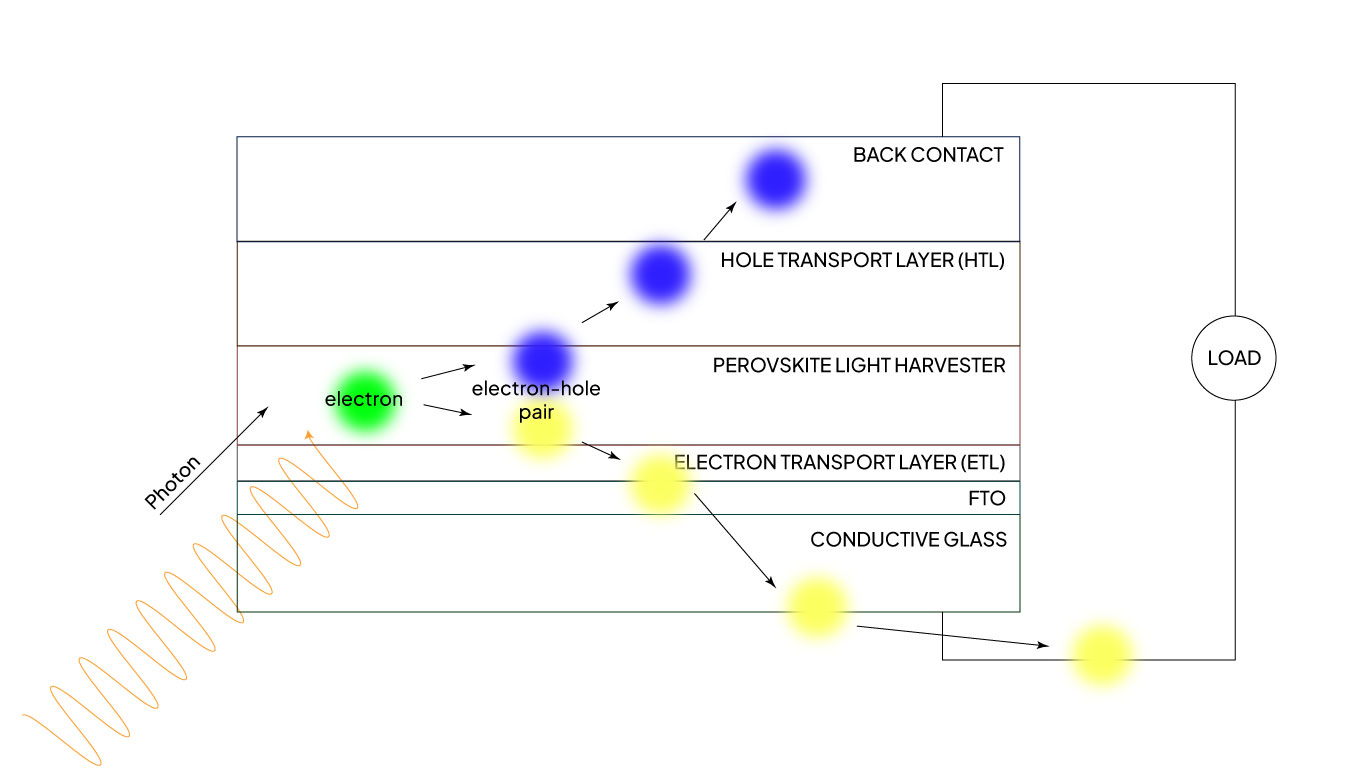
\includegraphics[width=14 cm]{img-content/psc-mechanism2.jpg}
\caption{Structure of a perovskite solar cell. Both glass (conductive) and Fluorine Tin Oxide (FTO) coats can also be collectively called front contact. A wire connecting back and front contact can be placed to allow the electron to flow\label{fig1}}
\end{figure}
